\documentclass[a4paper,12pt]{article}
\usepackage{../../synopsis/my_preamble}

\geometry{
    includehead,
    headsep=\baselineskip,
}

\usepackage{pgfplots}

\DeclareUnicodeCharacter{2212}{-}
\usepgfplotslibrary{groupplots,dateplot}
\usetikzlibrary{patterns,shapes.arrows}
\pgfplotsset{compat=newest}

\usepackage{graphicx}
\graphicspath{ {./img/} }

\pagestyle{fancy}
\fancyhf{}
\setlength{\headheight}{30pt}
\lhead{$\bm{\mathcal{H}}$\textbf{omework~\#5}\\\textbf{Graph~Theory}}
\rhead{\textbf{sltKaguya,~Group}\\\textbf{April~30~---~\today}}

\newcommand{\graph}[1][G]{\mathcal{#1}}

\newcommand{\op}[1]{\operatorname*{#1}}

\newcommand{\minDegree}[1]{\delta(#1)}
\newcommand{\maxDegree}[1]{\Delta(#1)}
\newcommand{\graphRadius}[1]{\op{rad}(#1)}
\newcommand{\graphDiameter}[1]{\op{diam}(#1)}
\newcommand{\graphGirth}[1]{\op{girth}(#1)}
\newcommand{\graphCenter}[1]{\op{center}(#1)}
\newcommand{\graphCentroid}[1]{\op{centroid}(#1)}
\newcommand{\vertexConnectivity}[1]{\varkappa(#1)}
\newcommand{\edgeConnectivity}[1]{\lambda(#1)}

\newcommand{\dist}[1]{\op{dist}(#1)}
\newcommand{\blockGraph}[1]{\op{B}(#1)}
\newcommand{\eccentricity}[1]{\varepsilon(#1)}

\begin{document}

\begin{tasks}
    \item The graph\footnote{Hereinafter, \enquote{graphs} are \enquote{simple, finite, undirected and unweighted}, unless stated otherwise.} of Europe $\graph^{*} = \langle V, E\rangle$ is defined as follows: each vertex $v \in V$ is a Europe country\footnote{\url{https://simple.wikipedia.org/wiki/List_of_European_countries} used as reference.}; two vertices are adjacent $(\{u, v\} \in E)$ if the corresponding countries share a land border. Let $\graph$ be the largest connected component of $\graph^{*}$.
    
    \begin{subtasks}
        \item Draw $\graph^{*}$ with the minimum number of intersecting edges.
            
        The graph was created in Python. More about creation can be found \href{https://github.com/sltKaguya/itmo/blob/wip/discr_math/05_graph_theory/05_homework.ipynb}{here}.

        A planar version of the graph (ugly):
        
            \begingroup
            \tikzset{every picture/.style={scale=1.5}}%
            % This file was created with tikzplotlib v0.10.1.
\begin{tikzpicture}

\definecolor{darkgray176}{RGB}{176,176,176}
\definecolor{steelblue31120180}{RGB}{31,120,180}

\begin{axis}[
hide x axis,
hide y axis,
scaled x ticks=manual:{}{\pgfmathparse{#1}},
scaled y ticks=manual:{}{\pgfmathparse{#1}},
tick align=outside,
x grid style={darkgray176},
xmajorticks=false,
xmin=-1.20721079691517, xmax=1.180646958012,
xtick style={color=black},
xticklabels={},
y grid style={darkgray176},
ymajorticks=false,
ymin=-0.327422879177378, ymax=0.409256640959726,
ytick style={color=black},
yticklabels={}
]
\path [draw=black]
(axis cs:-1,-0.263496143958869)
--(axis cs:-0.664095972579263,0.072407883461868);

\path [draw=black]
(axis cs:-1,-0.263496143958869)
--(axis cs:-0.937017994858612,-0.242502142245073);

\path [draw=black]
(axis cs:-1,-0.263496143958869)
--(axis cs:0.97343616109683,-0.263496143958869);

\path [draw=black]
(axis cs:-1,-0.263496143958869)
--(axis cs:-0.685089974293059,0.0304198800342759);

\path [draw=black]
(axis cs:-0.664095972579263,0.072407883461868)
--(axis cs:-0.664095972579263,0.00942587832047985);

\path [draw=black]
(axis cs:-0.664095972579263,0.072407883461868)
--(axis cs:-0.685089974293059,0.0304198800342759);

\path [draw=black]
(axis cs:-0.664095972579263,0.072407883461868)
--(axis cs:-0.622107969151671,0.0304198800342759);

\path [draw=black]
(axis cs:-0.937017994858612,-0.242502142245073)
--(axis cs:0.97343616109683,-0.263496143958869);

\path [draw=black]
(axis cs:-0.937017994858612,-0.242502142245073)
--(axis cs:-0.685089974293059,0.0304198800342759);

\path [draw=black]
(axis cs:-0.937017994858612,-0.242502142245073)
--(axis cs:-0.916023993144816,-0.221508140531277);

\path [draw=black]
(axis cs:0.97343616109683,-0.263496143958869)
--(axis cs:0.889460154241645,-0.200514138817481);

\path [draw=black]
(axis cs:0.97343616109683,-0.263496143958869)
--(axis cs:0.889460154241645,-0.179520137103685);

\path [draw=black]
(axis cs:0.97343616109683,-0.263496143958869)
--(axis cs:-0.916023993144816,-0.221508140531277);

\path [draw=black]
(axis cs:-0.685089974293059,0.0304198800342759)
--(axis cs:-0.664095972579263,0.00942587832047985);

\path [draw=black]
(axis cs:-0.685089974293059,0.0304198800342759)
--(axis cs:-0.916023993144816,-0.221508140531277);

\path [draw=black]
(axis cs:0.511568123393316,0.051413881748072)
--(axis cs:0.721508140531277,-0.0115681233933162);

\path [draw=black]
(axis cs:0.511568123393316,0.051413881748072)
--(axis cs:0.574550128534704,0.0934018851756641);

\path [draw=black]
(axis cs:0.721508140531277,-0.0115681233933162)
--(axis cs:0.427592116538132,0.00942587832047985);

\path [draw=black]
(axis cs:0.721508140531277,-0.0115681233933162)
--(axis cs:0.427592116538132,0.282347900599829);

\path [draw=black]
(axis cs:0.721508140531277,-0.0115681233933162)
--(axis cs:0.805484147386461,-0.0955441302485004);

\path [draw=black]
(axis cs:0.721508140531277,-0.0115681233933162)
--(axis cs:0.49057412167952,0.0304198800342759);

\path [draw=black]
(axis cs:0.721508140531277,-0.0115681233933162)
--(axis cs:0.574550128534704,0.11439588688946);

\path [draw=black]
(axis cs:0.721508140531277,-0.0115681233933162)
--(axis cs:0.574550128534704,0.0934018851756641);

\path [draw=black]
(axis cs:0.721508140531277,-0.0115681233933162)
--(axis cs:0.343616109682948,-0.0745501285347044);

\path [draw=black]
(axis cs:0.574550128534704,0.0934018851756641)
--(axis cs:0.574550128534704,0.072407883461868);

\path [draw=black]
(axis cs:-0.559125964010283,-0.0115681233933162)
--(axis cs:-0.30719794344473,0.345329905741217);

\path [draw=black]
(axis cs:-0.559125964010283,-0.0115681233933162)
--(axis cs:-0.622107969151671,0.0304198800342759);

\path [draw=black]
(axis cs:-0.30719794344473,0.345329905741217)
--(axis cs:-0.244215938303342,0.282347900599829);

\path [draw=black]
(axis cs:-0.30719794344473,0.345329905741217)
--(axis cs:-0.622107969151671,0.0304198800342759);

\path [draw=black]
(axis cs:-0.622107969151671,0.0304198800342759)
--(axis cs:-0.664095972579263,0.00942587832047985);

\path [draw=black]
(axis cs:0.259640102827764,-0.116538131962297)
--(axis cs:0.133676092544987,-0.0325621251071123);

\path [draw=black]
(axis cs:0.259640102827764,-0.116538131962297)
--(axis cs:0.427592116538132,0.282347900599829);

\path [draw=black]
(axis cs:0.259640102827764,-0.116538131962297)
--(axis cs:-0.790059982862039,-0.158526135389889);

\path [draw=black]
(axis cs:0.259640102827764,-0.116538131962297)
--(axis cs:0.805484147386461,-0.0955441302485004);

\path [draw=black]
(axis cs:0.259640102827764,-0.116538131962297)
--(axis cs:0.322622107969152,-0.0535561268209083);

\path [draw=black]
(axis cs:0.259640102827764,-0.116538131962297)
--(axis cs:0.175664095972579,-0.0955441302485004);

\path [draw=black]
(axis cs:0.259640102827764,-0.116538131962297)
--(axis cs:0.847472150814053,-0.137532133676093);

\path [draw=black]
(axis cs:0.259640102827764,-0.116538131962297)
--(axis cs:0.343616109682948,-0.0745501285347044);

\path [draw=black]
(axis cs:0.133676092544987,-0.0325621251071123)
--(axis cs:0.427592116538132,0.282347900599829);

\path [draw=black]
(axis cs:0.133676092544987,-0.0325621251071123)
--(axis cs:0.0916880891173951,-0.0535561268209083);

\path [draw=black]
(axis cs:0.133676092544987,-0.0325621251071123)
--(axis cs:0.175664095972579,-0.0955441302485004);

\path [draw=black]
(axis cs:0.427592116538132,0.282347900599829)
--(axis cs:0.427592116538132,0.00942587832047985);

\path [draw=black]
(axis cs:0.427592116538132,0.282347900599829)
--(axis cs:0.154670094258783,-0.0115681233933162);

\path [draw=black]
(axis cs:0.427592116538132,0.282347900599829)
--(axis cs:0.49057412167952,0.0304198800342759);

\path [draw=black]
(axis cs:0.427592116538132,0.282347900599829)
--(axis cs:0.469580119965724,0.051413881748072);

\path [draw=black]
(axis cs:0.427592116538132,0.282347900599829)
--(axis cs:0.0916880891173951,-0.0535561268209083);

\path [draw=black]
(axis cs:0.427592116538132,0.282347900599829)
--(axis cs:0.343616109682948,-0.0745501285347044);

\path [draw=black]
(axis cs:-0.790059982862039,-0.158526135389889)
--(axis cs:0.889460154241645,-0.179520137103685);

\path [draw=black]
(axis cs:-0.790059982862039,-0.158526135389889)
--(axis cs:-0.685089974293059,-0.0325621251071123);

\path [draw=black]
(axis cs:-0.790059982862039,-0.158526135389889)
--(axis cs:-0.916023993144816,-0.221508140531277);

\path [draw=black]
(axis cs:-0.790059982862039,-0.158526135389889)
--(axis cs:0.175664095972579,-0.0955441302485004);

\path [draw=black]
(axis cs:-0.790059982862039,-0.158526135389889)
--(axis cs:0.847472150814053,-0.137532133676093);

\path [draw=black]
(axis cs:-0.790059982862039,-0.158526135389889)
--(axis cs:-0.454155955441302,-0.0745501285347044);

\path [draw=black]
(axis cs:0.805484147386461,-0.0955441302485004)
--(axis cs:0.700514138817481,-0.0535561268209083);

\path [draw=black]
(axis cs:0.805484147386461,-0.0955441302485004)
--(axis cs:0.847472150814053,-0.137532133676093);

\path [draw=black]
(axis cs:0.805484147386461,-0.0955441302485004)
--(axis cs:0.343616109682948,-0.0745501285347044);

\path [draw=black]
(axis cs:0.805484147386461,-0.0955441302485004)
--(axis cs:0.721508140531277,-0.0325621251071123);

\path [draw=black]
(axis cs:0.322622107969152,-0.0535561268209083)
--(axis cs:0.343616109682948,-0.0745501285347044);

\path [draw=black]
(axis cs:0.175664095972579,-0.0955441302485004)
--(axis cs:0.0916880891173951,-0.0535561268209083);

\path [draw=black]
(axis cs:0.175664095972579,-0.0955441302485004)
--(axis cs:-0.454155955441302,-0.0745501285347044);

\path [draw=black]
(axis cs:0.847472150814053,-0.137532133676093)
--(axis cs:0.889460154241645,-0.179520137103685);

\path [draw=black]
(axis cs:-0.30719794344473,0.072407883461868)
--(axis cs:-0.0972579263067695,0.11439588688946);

\path [draw=black]
(axis cs:-0.30719794344473,0.072407883461868)
--(axis cs:-0.0762639245929734,0.0934018851756641);

\path [draw=black]
(axis cs:-0.30719794344473,0.072407883461868)
--(axis cs:0.0916880891173951,-0.0535561268209083);

\path [draw=black]
(axis cs:-0.30719794344473,0.072407883461868)
--(axis cs:-0.244215938303342,0.282347900599829);

\path [draw=black]
(axis cs:-0.30719794344473,0.072407883461868)
--(axis cs:-0.454155955441302,-0.0745501285347044);

\path [draw=black]
(axis cs:-0.0972579263067695,0.11439588688946)
--(axis cs:-0.244215938303342,0.135389888603256);

\path [draw=black]
(axis cs:-0.0972579263067695,0.11439588688946)
--(axis cs:-0.0762639245929734,0.0934018851756641);

\path [draw=black]
(axis cs:-0.0972579263067695,0.11439588688946)
--(axis cs:-0.244215938303342,0.282347900599829);

\path [draw=black]
(axis cs:-0.0762639245929734,0.0934018851756641)
--(axis cs:0.0916880891173951,-0.0535561268209083);

\path [draw=black]
(axis cs:-0.0762639245929734,0.0934018851756641)
--(axis cs:-0.244215938303342,0.282347900599829);

\path [draw=black]
(axis cs:0.0916880891173951,-0.0535561268209083)
--(axis cs:-0.244215938303342,0.282347900599829);

\path [draw=black]
(axis cs:0.0916880891173951,-0.0535561268209083)
--(axis cs:-0.454155955441302,-0.0745501285347044);

\path [draw=black]
(axis cs:-0.244215938303342,0.282347900599829)
--(axis cs:-0.244215938303342,0.135389888603256);

\path [draw=black]
(axis cs:-0.244215938303342,0.282347900599829)
--(axis cs:-0.139245929734362,0.156383890317052);

\path [draw=black]
(axis cs:-0.244215938303342,0.282347900599829)
--(axis cs:-0.20222793487575,0.177377892030848);

\path [draw=black]
(axis cs:-0.244215938303342,0.282347900599829)
--(axis cs:-0.454155955441302,-0.0745501285347044);

\path [draw=black]
(axis cs:-0.454155955441302,-0.0745501285347044)
--(axis cs:-0.685089974293059,-0.0535561268209083);

\path [draw=black]
(axis cs:-0.454155955441302,-0.0745501285347044)
--(axis cs:-0.685089974293059,-0.0325621251071123);

\path [draw=black]
(axis cs:0.427592116538132,0.00942587832047985)
--(axis cs:0.49057412167952,0.0304198800342759);

\path [draw=black]
(axis cs:0.427592116538132,0.00942587832047985)
--(axis cs:0.469580119965724,0.051413881748072);

\path [draw=black]
(axis cs:0.889460154241645,-0.200514138817481)
--(axis cs:0.889460154241645,-0.179520137103685);

\path [draw=black]
(axis cs:0.889460154241645,-0.200514138817481)
--(axis cs:-0.916023993144816,-0.221508140531277);

\path [draw=black]
(axis cs:0.889460154241645,-0.179520137103685)
--(axis cs:-0.916023993144816,-0.221508140531277);

\path [draw=black]
(axis cs:-0.916023993144816,-0.221508140531277)
--(axis cs:-0.664095972579263,0.00942587832047985);

\path [draw=black]
(axis cs:-0.916023993144816,-0.221508140531277)
--(axis cs:-0.685089974293059,-0.0325621251071123);

\path [draw=black]
(axis cs:-0.664095972579263,0.00942587832047985)
--(axis cs:-0.685089974293059,-0.0325621251071123);

\path [draw=black]
(axis cs:-0.685089974293059,-0.0325621251071123)
--(axis cs:-0.685089974293059,-0.0535561268209083);

\path [draw=black]
(axis cs:-0.139245929734362,0.156383890317052)
--(axis cs:-0.20222793487575,0.177377892030848);

\path [draw=black]
(axis cs:-0.139245929734362,0.156383890317052)
--(axis cs:-0.181233933161954,0.198371893744644);

\path [draw=black]
(axis cs:-0.20222793487575,0.177377892030848)
--(axis cs:-0.181233933161954,0.198371893744644);

\path [draw=black]
(axis cs:-0.244215938303342,-0.0115681233933162)
--(axis cs:-0.349185946872322,0.00942587832047985);

\addplot [draw=steelblue31120180, fill=steelblue31120180, mark=*, only marks]
table{%
x  y
-1 -0.263496143958869
-0.664095972579263 0.072407883461868
-0.937017994858612 -0.242502142245073
0.97343616109683 -0.263496143958869
-0.685089974293059 0.0304198800342759
0.511568123393316 0.051413881748072
0.721508140531277 -0.0115681233933162
0.574550128534704 0.0934018851756641
-0.559125964010283 -0.0115681233933162
-0.30719794344473 0.345329905741217
-0.622107969151671 0.0304198800342759
0.259640102827764 -0.116538131962297
0.133676092544987 -0.0325621251071123
0.427592116538132 0.282347900599829
-0.790059982862039 -0.158526135389889
0.805484147386461 -0.0955441302485004
0.322622107969152 -0.0535561268209083
0.175664095972579 -0.0955441302485004
0.847472150814053 -0.137532133676093
0.343616109682948 -0.0745501285347044
-0.30719794344473 0.072407883461868
-0.0972579263067695 0.11439588688946
-0.0762639245929734 0.0934018851756641
0.0916880891173951 -0.0535561268209083
-0.244215938303342 0.282347900599829
-0.454155955441302 -0.0745501285347044
0.427592116538132 0.00942587832047985
0.49057412167952 0.0304198800342759
0.469580119965724 0.051413881748072
0.889460154241645 -0.200514138817481
0.889460154241645 -0.179520137103685
-0.916023993144816 -0.221508140531277
-0.664095972579263 0.00942587832047985
-0.685089974293059 -0.0325621251071123
-0.30719794344473 0.051413881748072
0.154670094258783 -0.0115681233933162
-0.244215938303342 0.135389888603256
-0.139245929734362 0.156383890317052
-0.20222793487575 0.177377892030848
-0.181233933161954 0.198371893744644
0.574550128534704 0.11439588688946
-0.328191945158526 0.0304198800342759
-0.244215938303342 -0.0115681233933162
-0.349185946872322 0.00942587832047985
0.700514138817481 -0.0535561268209083
0.721508140531277 -0.0325621251071123
-0.391173950299914 -0.0325621251071123
-0.685089974293059 -0.0535561268209083
0.574550128534704 0.072407883461868
};
\draw (axis cs:-1,-0.263496143958869) node[
  scale=0.6,
  text=black,
  rotate=0.0
]{Albania};
\draw (axis cs:-0.664095972579263,0.072407883461868) node[
  scale=0.6,
  text=black,
  rotate=0.0
]{Greece};
\draw (axis cs:-0.937017994858612,-0.242502142245073) node[
  scale=0.6,
  text=black,
  rotate=0.0
]{Kosovo};
\draw (axis cs:0.97343616109683,-0.263496143958869) node[
  scale=0.6,
  text=black,
  rotate=0.0
]{Montenegro};
\draw (axis cs:-0.685089974293059,0.0304198800342759) node[
  scale=0.6,
  text=black,
  rotate=0.0
]{North Macedonia};
\draw (axis cs:0.511568123393316,0.051413881748072) node[
  scale=0.6,
  text=black,
  rotate=0.0
]{Andorra};
\draw (axis cs:0.721508140531277,-0.0115681233933162) node[
  scale=0.6,
  text=black,
  rotate=0.0
]{France};
\draw (axis cs:0.574550128534704,0.0934018851756641) node[
  scale=0.6,
  text=black,
  rotate=0.0
]{Spain};
\draw (axis cs:-0.559125964010283,-0.0115681233933162) node[
  scale=0.6,
  text=black,
  rotate=0.0
]{Armenia};
\draw (axis cs:-0.30719794344473,0.345329905741217) node[
  scale=0.6,
  text=black,
  rotate=0.0
]{Georgia};
\draw (axis cs:-0.622107969151671,0.0304198800342759) node[
  scale=0.6,
  text=black,
  rotate=0.0
]{Turkey};
\draw (axis cs:0.259640102827764,-0.116538131962297) node[
  scale=0.6,
  text=black,
  rotate=0.0
]{Austria};
\draw (axis cs:0.133676092544987,-0.0325621251071123) node[
  scale=0.6,
  text=black,
  rotate=0.0
]{Czech Republic};
\draw (axis cs:0.427592116538132,0.282347900599829) node[
  scale=0.6,
  text=black,
  rotate=0.0
]{Germany};
\draw (axis cs:-0.790059982862039,-0.158526135389889) node[
  scale=0.6,
  text=black,
  rotate=0.0
]{Hungary};
\draw (axis cs:0.805484147386461,-0.0955441302485004) node[
  scale=0.6,
  text=black,
  rotate=0.0
]{Italy};
\draw (axis cs:0.322622107969152,-0.0535561268209083) node[
  scale=0.6,
  text=black,
  rotate=0.0
]{Liechtenstein};
\draw (axis cs:0.175664095972579,-0.0955441302485004) node[
  scale=0.6,
  text=black,
  rotate=0.0
]{Slovakia};
\draw (axis cs:0.847472150814053,-0.137532133676093) node[
  scale=0.6,
  text=black,
  rotate=0.0
]{Slovenia};
\draw (axis cs:0.343616109682948,-0.0745501285347044) node[
  scale=0.6,
  text=black,
  rotate=0.0
]{Switzerland};
\draw (axis cs:-0.30719794344473,0.072407883461868) node[
  scale=0.6,
  text=black,
  rotate=0.0
]{Belarus};
\draw (axis cs:-0.0972579263067695,0.11439588688946) node[
  scale=0.6,
  text=black,
  rotate=0.0
]{Latvia};
\draw (axis cs:-0.0762639245929734,0.0934018851756641) node[
  scale=0.6,
  text=black,
  rotate=0.0
]{Lithuania};
\draw (axis cs:0.0916880891173951,-0.0535561268209083) node[
  scale=0.6,
  text=black,
  rotate=0.0
]{Poland};
\draw (axis cs:-0.244215938303342,0.282347900599829) node[
  scale=0.6,
  text=black,
  rotate=0.0
]{Russia};
\draw (axis cs:-0.454155955441302,-0.0745501285347044) node[
  scale=0.6,
  text=black,
  rotate=0.0
]{Ukraine};
\draw (axis cs:0.427592116538132,0.00942587832047985) node[
  scale=0.6,
  text=black,
  rotate=0.0
]{Belgium};
\draw (axis cs:0.49057412167952,0.0304198800342759) node[
  scale=0.6,
  text=black,
  rotate=0.0
]{Luxembourg};
\draw (axis cs:0.469580119965724,0.051413881748072) node[
  scale=0.6,
  text=black,
  rotate=0.0
]{Netherlands};
\draw (axis cs:0.889460154241645,-0.200514138817481) node[
  scale=0.6,
  text=black,
  rotate=0.0
]{Bosnia and Herzegovina};
\draw (axis cs:0.889460154241645,-0.179520137103685) node[
  scale=0.6,
  text=black,
  rotate=0.0
]{Croatia};
\draw (axis cs:-0.916023993144816,-0.221508140531277) node[
  scale=0.6,
  text=black,
  rotate=0.0
]{Serbia};
\draw (axis cs:-0.664095972579263,0.00942587832047985) node[
  scale=0.6,
  text=black,
  rotate=0.0
]{Bulgaria};
\draw (axis cs:-0.685089974293059,-0.0325621251071123) node[
  scale=0.6,
  text=black,
  rotate=0.0
]{Romania};
\draw (axis cs:-0.30719794344473,0.051413881748072) node[
  scale=0.6,
  text=black,
  rotate=0.0
]{Cyprus};
\draw (axis cs:0.154670094258783,-0.0115681233933162) node[
  scale=0.6,
  text=black,
  rotate=0.0
]{Denmark};
\draw (axis cs:-0.244215938303342,0.135389888603256) node[
  scale=0.6,
  text=black,
  rotate=0.0
]{Estonia};
\draw (axis cs:-0.139245929734362,0.156383890317052) node[
  scale=0.6,
  text=black,
  rotate=0.0
]{Finland};
\draw (axis cs:-0.20222793487575,0.177377892030848) node[
  scale=0.6,
  text=black,
  rotate=0.0
]{Norway};
\draw (axis cs:-0.181233933161954,0.198371893744644) node[
  scale=0.6,
  text=black,
  rotate=0.0
]{Sweden};
\draw (axis cs:0.574550128534704,0.11439588688946) node[
  scale=0.6,
  text=black,
  rotate=0.0
]{Monaco};
\draw (axis cs:-0.328191945158526,0.0304198800342759) node[
  scale=0.6,
  text=black,
  rotate=0.0
]{Iceland};
\draw (axis cs:-0.244215938303342,-0.0115681233933162) node[
  scale=0.6,
  text=black,
  rotate=0.0
]{Ireland};
\draw (axis cs:-0.349185946872322,0.00942587832047985) node[
  scale=0.6,
  text=black,
  rotate=0.0
]{United Kingdom};
\draw (axis cs:0.700514138817481,-0.0535561268209083) node[
  scale=0.6,
  text=black,
  rotate=0.0
]{San Marino};
\draw (axis cs:0.721508140531277,-0.0325621251071123) node[
  scale=0.6,
  text=black,
  rotate=0.0
]{Vatican City};
\draw (axis cs:-0.391173950299914,-0.0325621251071123) node[
  scale=0.6,
  text=black,
  rotate=0.0
]{Malta};
\draw (axis cs:-0.685089974293059,-0.0535561268209083) node[
  scale=0.6,
  text=black,
  rotate=0.0
]{Moldova};
\draw (axis cs:0.574550128534704,0.072407883461868) node[
  scale=0.6,
  text=black,
  rotate=0.0
]{Portugal};
\end{axis}

\end{tikzpicture}

            \endgroup
        \newpage
        A prettier version (but unfinished):

            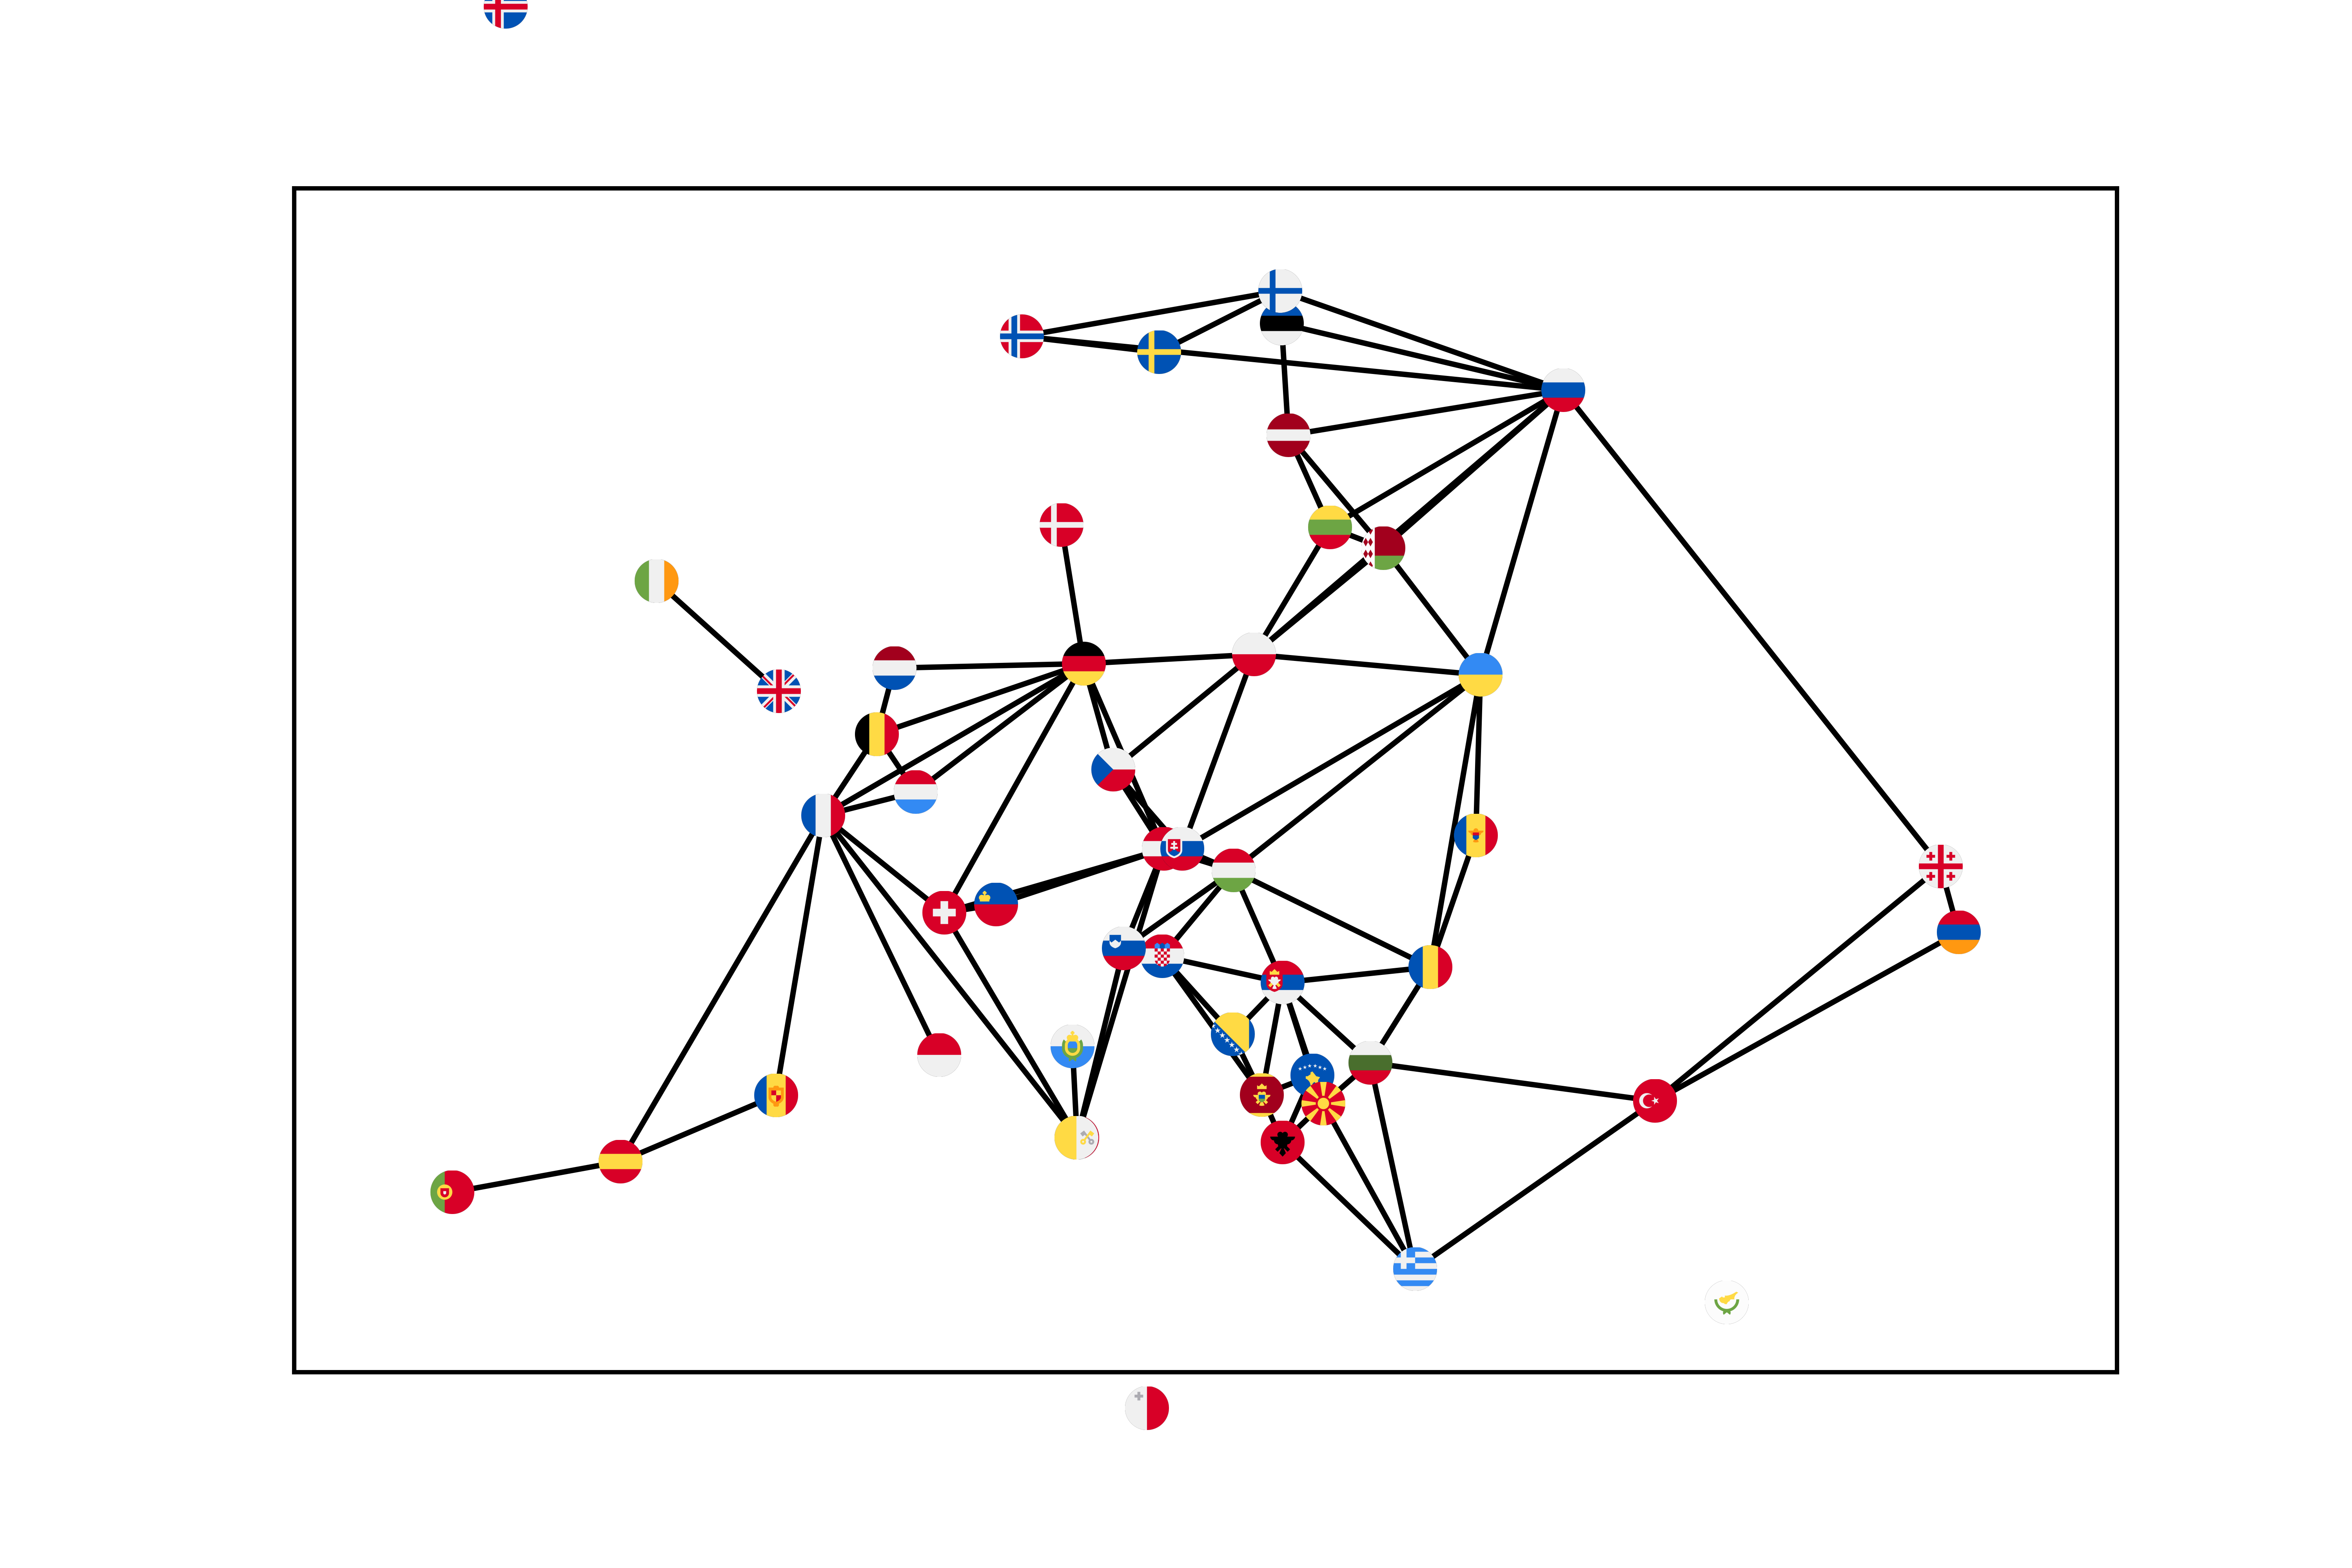
\includegraphics{Eurograph}
        \item Find $\card{V}$, $\card{E}$, $\minDegree{\graph}$, $\maxDegree{\graph}$, $\graphRadius{\graph}$, $\graphDiameter{\graph}$, $\graphGirth{\graph}$, $\graphCenter{\graph}$, $\vertexConnectivity{\graph}$, $\edgeConnectivity{\graph}$.

        $\card{V} = 49$, $\card{E} = 92$
        \item Find the minimum vertex coloring $Z: V \to \sets{N}$ of $\graph$.
        
        \item Find the minimum edge coloring $X: E \to \sets{N}$ of $\graph$.
        
        \item Find the maximum clique $Q \subseteq V$ of $\graph$.

        \item Find the maximum stable set $S \subseteq V$ of $\graph$.
        
        \item Find the maximum matching $M \subseteq E$ of $\graph$.
        
        \item Find the minimum vertex cover $R \subseteq V$ of $\graph$.
        
        \item Find the minimum edge cover $F \subseteq E$ of $\graph$.
        
        \item Find the shortest closed walk $W$ that visits every vertex of $\graph$.
        
        \item Find the shortest closed walk $U$ that visits every edge of $\graph$.
        
        \item Find all biconnected components (blocks) and draw the block-cut tree of $\graph^{*}$.
        
        \item Find all 2-edge-connected components of $\graph^{*}$.
        
        \item Construct an SPQR tree of the largest biconected component of $\graph^{*}$.
        
        \item Add the weight function $w: E \to \sets{R}$ denoting the distance between capitals. Find the minimum (\textit{w.r.t.} the total weight of edges) spanning tree $T$ for the largest connected component of the weighted Europe graph $\graph^{*}_{w} = (V, E, w)$.
        
        \item Find $\graphCentroid{T}$ (\textit{w.r.t.} the edge weight function $w$).
        
        \item Construct the Prüfer code for $T$.
    \end{subtasks}

    \item Prove \emph{rigorously} the following theorems:
    
    \begin{theorem}[Triangle Inequality]
        For any connected graph $G = \angled{V, E}$:
        $$\forall x, y, z \in V: \dist{x, y} + \dist{y, z} \geq \dist{x, z}$$
    \end{theorem}

    \begin{theorem}[Tree]
        A connected graph $G = \angled{V, E}$ is a tree (\ie acyclic graph) \emph{iff} $\card{E} = \card{V} - 1$.
    \end{theorem}

    \begin{theorem}[Whitney]
        For any graph $G:$ $\vertexConnectivity{G} \leq \edgeConnectivity{G} \leq \minDegree{G}$.
    \end{theorem}

    \begin{theorem}[Chartrand]
        For a connected graph $G = \angled{V, E}$: if $\minDegree{G} \geq \floor{\frac{\card{V}}{2}}$, then $\edgeConnectivity{G} = \minDegree{G}$. 
    \end{theorem}

    \begin{theorem}[Menger]
        For any pair of non-adjacent vertices $u$ and $v$ in an undirected graph, the size of the minimum \textit{vertex cut} is equal to the maximum number of pairwise \textit{internally vertex-disjoint paths} from $u$ to $v$.
    \end{theorem}

    \begin{theorem}[Harary]
        Every block of a block graph\footnote{A block graph $H = \blockGraph{G}$ is an intersection graph of all blocks (biconnected components) of $G$, \ie each vertex $v \in V(H)$ corresponds to a block of $G$, and there is an edge $\{v, u\} \in E(H)$ iff \enquote{blocks} $v$ and $u$ share a cut vertex.} is a clique.
    \end{theorem}

\end{tasks}

\end{document}